\documentclass{article}
\usepackage{harvard}
\usepackage{hyperref}
\usepackage{graphics}
\usepackage{amsmath}
\usepackage{indentfirst}
\usepackage[utf8]{inputenc}
\usepackage[top=1in, bottom=1in, left=1in, right=1in]{geometry}
\DeclareMathOperator{\var}{var}
% \VignetteIndexEntry{Using PwrGSD}
\usepackage{/usr/local/lib64/R/share/texmf/Sweave}
\begin{document}


\title{Comparing the performance of a panel of candidate interim monitoring schemes over
  a range of hypothetical trial scenarios, using cpd.PwrGSD (Version 1.1)}
\author{Grant Izmirlian}
\maketitle

\section{Introduction}
The selection of a test statistic and boundary construction method in the design of an
interim monitoring plan is done by computing several operating characteristics, such as
power, expected duration and relative risks at the stopping boundaries, for each candidate
plan under a variety of hypothetical trial scenarios and under various options for
boundary construction. Thus one wishes to optimize, in the sense of best overall
performance over a range of trial scenarios, these operating characteristics with respect
to the variables over which one has control.  There is usually not a unique optimal
choice, especially if the user is realistic about the range of trial scenarios. However,
if one chooses a balance of behavior under favorable scenarios and under unfavorable
scenarios, and the investigation has appealed to a rich enough variety of appropriate 
choices, an acceptible monitoring scheme will be found. 


In order to understand this vignette, you should familiarize
yourself with the function {\bf PwrGSD} which computes these operating characteristics
for a specification of the trial scenario (which admits non-proportional hazards
alternatives through the specification of control and intervention arm specific piecewise
constant hazard rates for the main event, censoring, and two modes of non-compliance),
choice of test statistic and choice of boundary construction method. Refer to the help
pages by typing \verb`?`{\bf PwrGSD} within R. 

The {\bf cpd.PwrGSD} function and its related class provide a infrastructure whereby the
behavior of the above-mentioned operating characteristics as the choice of statistic,
boundary construction method (design space) and hypothetical trial scenarios (outcome
space) vary can be flexibly determined and then conveniently summarized.  To summarize the
idea, note that the function {\bf cpd.PwrGSD} takes as its sole argument a data.frame, the
descriptor, with a complete specification of a point in the design by outcome space per
line and creates as output, a skeleton object of class {\bf cpd.PwrGSD} as its output.
The most important component of this output (a list of class {\bf cpd.PwrGSD}) is the
component {\bf Elements}. This starts life as a list, with NULL components, of length
equal to the number of rows of the descriptor data.frame. The functionality of this
infrastructure to summarize, i.e. in the form of a trellis plot, for example, comes from
the implicit cross-linking between the components of {\bf Elements} and the rows of the
descriptor data.frame.  The flexibility of this infrastructure owes to the fact that it is
completely user determined.  The exact meaning of this will become apparent in the example
below. The full extent of the capabilities can be well understood by absorbing the
capabilities of {\bf PwrGSD}, which computes operating characteristics for a single point
in design by outcome space.

In order to set up a compound object of class {\bf cpd.PwrGSD} we first construct a base
case: a two arm trial randomized in just under eight years with a maximum of 20 years of
follow-up. We compute power at a specific alternative, {\bf rhaz}, under an interim
analysis plan with roughly one analysis per year, some crossover between intervention and
control arms, with Efficacy and futility boundaries constructed via the Lan-Demets
procedure with O'Brien-Fleming spending on the hybrid scale. We investigate the behavior of
three weighted log-rank statistics: (i) the Fleming-Harrington(0,1) statistic,
(ii) a stopped version of the F-H(0,1) statistic capped off at 10 years, and
(iii) the deterministic weighting function with linear increase between time 0
and time 10 with constant weight thereafter.

\begin{Schunk}
\begin{Sinput}
> tlook <- c(7.14, 8.14, 9.14, 10.14, 10.64, 11.15, 12.14, 
+     13.14, 14.14, 15.14, 16.14, 17.14, 18.14, 19.14, 
+     20.14)
> t0 <- 0:19
> h0 <- c(rep(0.000373, 2), rep(0.000745, 3), rep(0.00149, 
+     15))
> rhaz <- c(1, 0.9125, 0.8688, 0.7814, 0.6941, 0.6943, 
+     0.6072, 0.5202, 0.4332, 0.652, 0.6524, 0.6527, 0.653, 
+     0.6534, 0.6537, 0.6541, 0.6544, 0.6547, 0.6551, 0.6554)
> hc <- c(rep(0.0105, 2), rep(0.0209, 3), rep(0.0419, 15))
> hd1B <- c(0.1109, 0.1381, 0.1485, 0.1637, 0.2446, 0.2497, 
+     0)
\end{Sinput}
\end{Schunk}

\begin{Schunk}
\begin{Sinput}
> library(PwrGSD)
> test.example <- PwrGSD(EfficacyBoundary = LanDemets(alpha = 0.05, 
+     spending = ObrienFleming), FutilityBoundary = LanDemets(alpha = 0.1, 
+     spending = ObrienFleming), RR.Futility = 0.82, sided = "<", 
+     method = "A", accru = 7.73, accrat = 9818.65, tlook = tlook, 
+     tcut0 = t0, h0 = h0, tcut1 = t0, rhaz = rhaz, tcutc0 = t0, 
+     hc0 = hc, tcutc1 = t0, hc1 = hc, tcutd0B = c(0, 13), 
+     hd0B = c(0.04777, 0), tcutd1B = 0:6, hd1B = hd1B, 
+     noncompliance = crossover, gradual = TRUE, WtFun = c("FH", 
+         "SFH", "Ramp"), ppar = c(0, 1, 0, 1, 10, 10))
\end{Sinput}
\end{Schunk}

Now {\bf test.example}, containing the computed operating characteristics
corresponding to our ``base case'' single point in design by outcome space in
the form of the resulting call to {\bf PwrGSD}.  Then we (the user) decide
how we wish to explore the design by outcome space by determining which pieces
of the picture we want to range over.  In the following we vary (i) the
alternative hypothesis by stipulating 9 values of the maximum effect, (ii) the
censoring amount by stipulating 3 values, and (iii) the boundary construction
method, as two efficacy boundary construction methods: Lan-Demets with
Obrien-Fleming spending and stochastic curtailment. Each of these will be
incorporated as a simple modification to the base case above.  

First, the vector of possible maximum effects for varying the alternative hypothesis:
\begin{Schunk}
\begin{Sinput}
> max.effect <- 0.8 + 0.05 * (0:8)
> n.me <- length(max.effect)
\end{Sinput}
\end{Schunk}

Next the vector of censoring amounts:
\begin{Schunk}
\begin{Sinput}
> cens.amt <- 0.75 + 0.25 * (0:2)
> n.ca <- length(cens.amt)
\end{Sinput}
\end{Schunk}

Finally the two methods of efficacy boundary construction: Lan-Demets method
with O'Brien-Fleming spending verus stochastic curtailment:  
\begin{Schunk}
\begin{Sinput}
> Eff.bound.choice <- 1:2
> ebc.nms <- c("LanDemets(alpha=0.05, spending=ObrienFleming)", 
+     "SC(alpha=0.05, crit=0.90)")
> n.ec <- length(Eff.bound.choice)
\end{Sinput}
\end{Schunk}

Next we create the descriptor data.frame, with one line corresponding to each
of the possible 9 * 3 * 2 possible choices.  This is done in the following line.
\begin{Schunk}
\begin{Sinput}
> descr <- as.data.frame(cbind(Eff.bound.choice = rep(Eff.bound.choice, 
+     each = n.ca * n.me), cens.amt = rep(rep(cens.amt, 
+     each = n.me), n.ec), max.effect = rep(max.effect, 
+     n.ec * n.ca)))
> descr$Eff.bound.choice <- ebc.nms[descr$Eff.bound.choice]
\end{Sinput}
\end{Schunk}

Now the descriptor data.frame, {\bf descr} contains one row for each combination of the
levels of the user defined selection variables, {\bf Eff.bound.choice}, {\bf max.effect}
and  {\bf cens.amt}. Keep in mind that the names and number of these variables is 
arbitrary. Next we create a skeleton {\bf cpd.PwrGSD} object with a call to
the function {\bf cpd.PwrGSD} with argument {\bf descr}

\begin{Schunk}
\begin{Sinput}
> test.example.set <- cpd.PwrGSD(descr)
\end{Sinput}
\end{Schunk}

Now, the newly created object, of class {\bf cpd.PwrGSD}, contains an element
{\bf descr}, a component {\bf date}, the date created and a component
{\bf Elements}, an empty list of length equal to the number of rows in
{\bf descr}.  Next we do the computation in a loop over the rows of
{\bf descr}.  Inside the loop we execute the following steps for each $k$. 
In the first line, we copy the original call to the current call,
{\bf Elements}\verb`[[k]]$call`. In the second line, we use the efficacy boundary
choice in the kth row of {\bf descr} to set the efficacy boundary choice in
the current call. In the third line, we derive the {\bf rhaz} defined by the
selection variable {\bf max.effect} in the kth row of {\bf descr} and use
this to set the {\bf rhaz} component of the current call. In the fourth line,
we derive the censoring components from the selection variable {\bf cens.amt}
in the kth row of {\bf descr} and place that result into the current call.
In this manner we have constructed a call to {\bf PwrGSD} that corresponds
exactly to the selection variable values in row $k$ of {\bf descr}. The
computation is done by calling {\bf update}:

\begin{Schunk}
\begin{Sinput}
> n.descr <- nrow(descr)
> for (k in 1:n.descr) {
+     test.example.set$Elements[[k]]$call <- test.example$call
+     test.example.set$Elements[[k]]$call$EfficacyBoundary <- parse(text = as.character(descr[k, 
+         "Eff.bound.choice"]))[[1]]
+     test.example.set$Elements[[k]]$call$rhaz <- exp(descr[k, 
+         "max.effect"] * log(rhaz))
+     test.example.set$Elements[[k]]$call$hc0 <- descr[k, 
+         "cens.amt"] * hc
+     test.example.set$Elements[[k]]$call$hc1 <- descr[k, 
+         "cens.amt"] * hc
+     test.example.set$Elements[[k]] <- update(test.example.set$Elements[[k]])
+ }
\end{Sinput}
\end{Schunk}

The functionality of this cross-linked list {\bf PwrGSD} elements and a
descriptor data.frame is the ability to extract subsets of this list through
the specification of subsets of the descriptor data.frame.  For example
the following creates a new {\bf cpd.PwrGSD} object by subsetting on
the selection variables in {\bf descr} as the first line below.

\begin{Schunk}
\begin{Sinput}
> test.example.subset <- Elements(test.example.set, subset = (substring(Eff.bound.choice, 
+     1, 9) == "LanDemets" & max.effect >= 1))
\end{Sinput}
\end{Schunk}

The plot method for {\bf cpd.PwrGSD} produces trellised stacked plots of
power and type II error at each analysis versus the magnitude of effect
conditioned on the values of two other descriptor variables. 

This is done via a formula argument of the form \verb`~ x | a` or 
\verb`~ x | a*b` which specify, a stacked plot of power and type II error as the magnitude
of effect, $x$ varies, that is conditioned on values of $a$ alone, in the
first case, and $a$ by $b$ in the second case, respectively. Subsetting is
also allowed.  In the first plot, \ref{fig:LanDemets}, we have subsetted to
the elements having Lan-Demets boundaries while in the second plot,
\ref{fig:StochCurt}, we have subsetted to the elements having boundaries
created via stochastic curtailment.

\begin{Schunk}
\begin{Sinput}
> plot(test.example.set, formula = ~max.effect | stat * 
+     cens.amt, subset = (substring(Eff.bound.choice, 1, 
+     9) == "LanDemets"))
\end{Sinput}
\end{Schunk}

\begin{Schunk}
\begin{Sinput}
> plot(test.example.set, formula = ~max.effect | stat * 
+     cens.amt, subset = (substring(Eff.bound.choice, 1, 
+     2) == "SC"))
\end{Sinput}
\end{Schunk}

\begin{figure}
\begin{center}
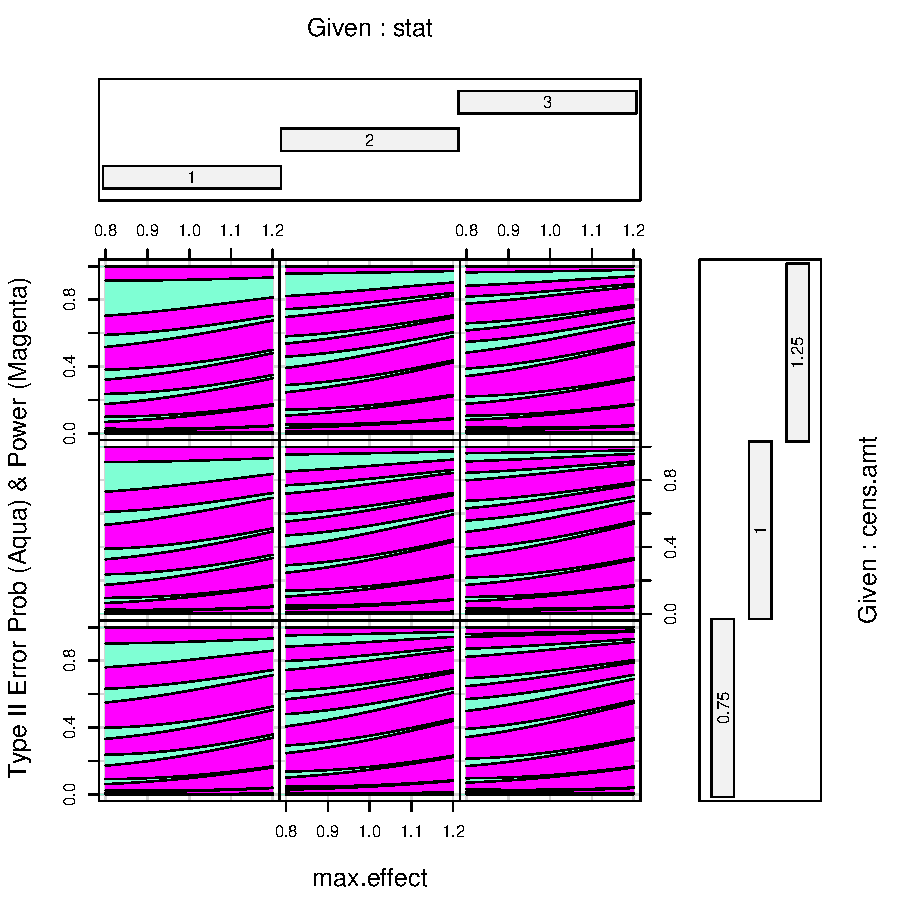
\includegraphics{cpd-PwrGSD-vignette-1-fig1-LanDemets}
\end{center}
\caption{Power (magenta) and type II error (cyan) at each analysis versus the
  maximum benefit. Lan-Demets efficacy and futility boundary using
  Obrien-Fleming spending.}
\label{fig:LanDemets}
\end{figure}

\begin{figure}
\begin{center}
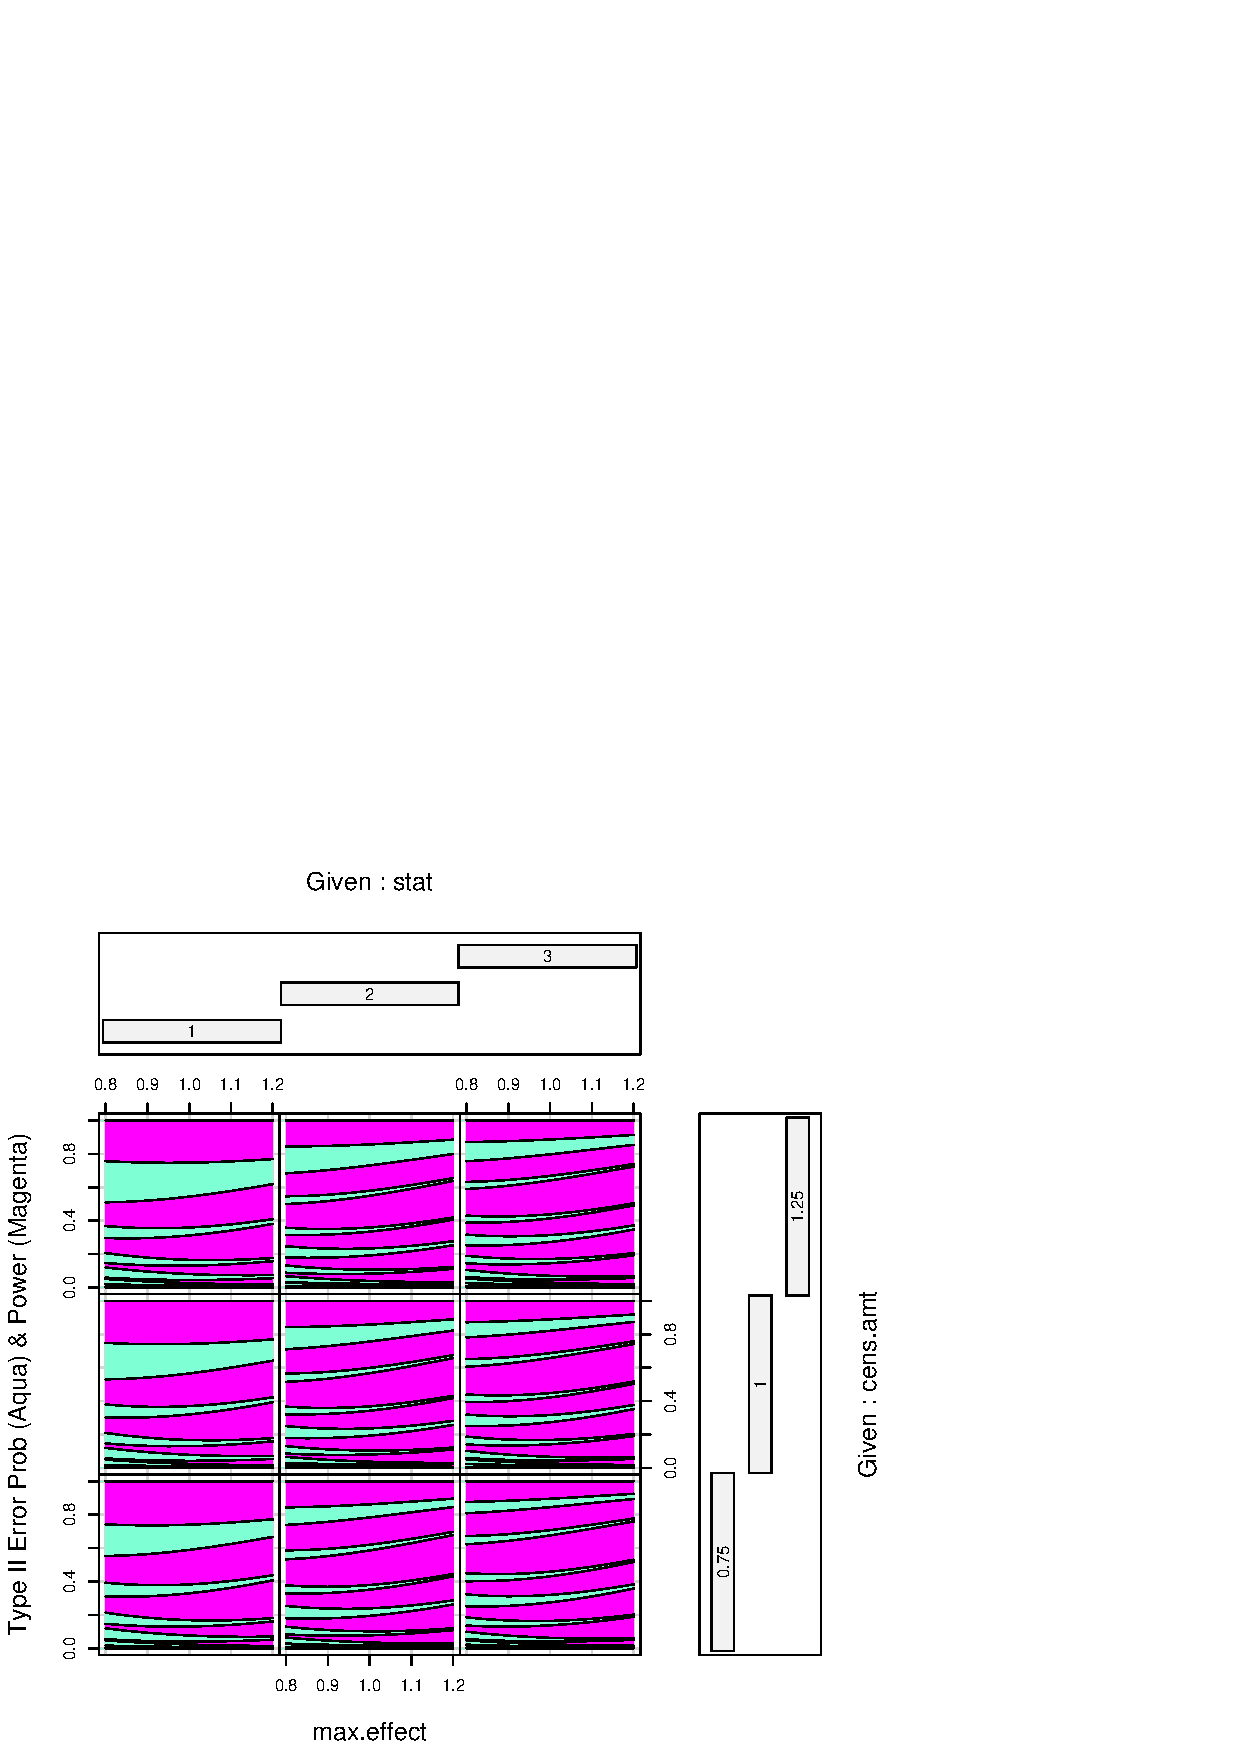
\includegraphics{cpd-PwrGSD-vignette-1-fig2-StochCurt}
\end{center}
\caption{Power (magenta) and type II error (cyan) at each analysis versus the
  maximum benefit. Efficacy boundary constructed via stochastic curtailment,
  Lan-Demets futility boundary using Obrien-Fleming spending.}
\label{fig:StochCurt}
\end{figure}

Notice the appearance of the selection variable {\bf stat} which was not defined
in the dataset {\bf descr}.  Recall that each single {\bf PwrGSD} object can
contain results for a list of test statistics, as in the example shown here
where we have results on three statistics per component of {\bf Elements}.
For this reason the variable {\bf stat} can be also be referenced in the
{\bf subset} or {\bf formula} arguments of calls to this {\bf plot} method.
\end{document}
